\documentclass[12pt,twoside]{report}
\usepackage[spanish,es-tabla]{babel}
\usepackage[a4paper]{geometry}

\usepackage{graphicx}               % Para incluir imágenes
\usepackage{amsmath}                % Para el manejo de matemáticas
\usepackage{url}
\usepackage{array}					% Para ajustar el texto en la celda
\usepackage{tabularx}
\usepackage{lipsum}
\usepackage{enumitem}
\usepackage{listings}
\usepackage{xcolor}
\usepackage{algorithm}
\usepackage{algpseudocode}
\usepackage{amssymb}

\lstdefinestyle{pythonstyle}{
	language=Python,
	basicstyle=\ttfamily\small,
	keywordstyle=\color{blue}\bfseries,
	commentstyle=\color{gray},
	stringstyle=\color{red},
	numbers=left,
	numberstyle=\tiny,
	stepnumber=1,
	frame=single,
	backgroundcolor=\color{lightgray!20},
	tabsize=4,
	showstringspaces=false,
	breaklines=true,        % Permite que las líneas largas se dividan
	linewidth=\linewidth    % Autoajuste al ancho del contenedor
}

% Opening
\title{Solución de problemas mediante recocido simulado}
\author{Erick Jesse Angeles López}


% Definir un comando para palabras clave
\newcommand{\keywords}[1]{%
	\begin{center}
		\textbf{Palabras clave:} #1
	\end{center}
}

\renewcommand{\baselinestretch}{1}
\setcounter{page}{1}
\setlength{\textheight}{21.6cm}
\setlength{\textwidth}{14cm}
\setlength{\oddsidemargin}{1cm}
\setlength{\evensidemargin}{1cm}
\pagestyle{myheadings}
\thispagestyle{empty}
\markboth{\small{Ángeles López Erick Jesse}}{\small{Algoritmos geneticos}}
\date{}

\begin{document}
	
	\begin{center}
		
		% Contenido izquierdo - Imagen
		\begin{minipage}{0.17\textwidth}
			\centering
			
\includegraphics[width=0.7\textwidth]{img/cic_logo.png} % Ajusta esta línea
		\end{minipage}
		\begin{minipage}{.55\textwidth}
			\centering
			{\Large Instituto Politécnico Nacional}\\
			{\Large Escuela Superior de Cómputo}\\
			{\Large Centro de Investigación en Computación}
		\end{minipage}
		\begin{minipage}{0.17\textwidth}
			\centering
			
\includegraphics[width=0.9\textwidth]{img/escom_logo} % Ajusta esta línea
		\end{minipage}			
	\end{center}
	
	
	\centerline{\bf Ingeniería en Inteligencia Artificial, Metaheuristicas}
	
	\centerline{\bf Fecha: \today}
	
	\centerline{}
	
	%\centerline{}
	
	
	\begin{center}
		\Large{\textsc{Algoritmos genéticos}} 
	\end{center}
	\centerline{}
	\centerline{\bf {\textit{Presenta}}}
	\centerline{}
	\centerline{\bf {Angeles López Erick Jesse\footnote{eangelesl1700@alumno.ipn.mx}}}
	\centerline{}
	\centerline{}
	\centerline{\bf {Disponible en:}}
	\centerline{\text{\url{github.com/JesseAngeles/Metaheuristicas}}}
	
	
	
	\newtheorem{Theorem}{\quad Theorem}[section]
	
	\newtheorem{Definition}[Theorem]{\quad Definition}
	
	\newtheorem{Corollary}[Theorem]{\quad Corollary}
	
	\newtheorem{Lemma}[Theorem]{\quad Lemma}
	
	\newtheorem{Example}[Theorem]{\quad Example}
	
	\bigskip
	
	\bigskip
	
	\begin{abstract} 
		Se describe el comportamiento de los algoritmos geneticos para resolver problemas de optimización local.
	\end{abstract}
	
	\keywords{Algoritmo, Algoritmo genético, Resultado óptimo}
	
	\clearpage
	
	\tableofcontents
	\clearpage
	
	\chapter*{Introducción}
	\addcontentsline{toc}{chapter}{Introducción}
	
	\chapter{Algoritmo genético}

\section{Evolución natural}

La evolución, en relación con la genómica, es el proceso por el cual los organismos vivos cambian con el tiempo a través de cambios en el genoma, esto cambios provocan individuos con rasgos alterados que afectan su supervivencia. Los supervivientes se reproducen y trasmiten estos genes alterados, los cambios que atentan contra la supervivencia de algún individuo, impide la reproducción del mismo \cite{evolucion}.

En la naturaleza, para que exista un proceso evolutivo se deben cumplir las siguientes condiciones:
\begin{itemize}
	\item Una entidad o individuo con la capacidad de reproducción.
	\item Una población de dichos individuos.
	\item Diferencias entre los individuos de la población.
	\item La variedad es un factor que determina el nivel de supervivencia de ese individuo.
\end{itemize}

La evolución afecta los cromosomas, estos son estructuras que transporta la información genómica de una célula a otra, y es mediante la reproducción en donde se combinan los cromosomas de los padres para formar nuevas estructuras \cite{evolucion_2, cromosoma}.

\section{Evolución artificial}

Los algoritmos genéticos simulan el comportamiento evolutivo de una población en donde los mas aptos heredan sus genes a las nuevas generaciones para obtener nuevos resultados.  Este proceso tiene los siguientes pasos:
\begin{itemize}
	\item \textbf{Selección}: Se seleccionan las parejas (o grupos) de individuos de la población con las mejores aptitudes. Este conjunto serán los padres de la nueva generación.
	
	\item \textbf{Cruza}: Se realiza una combinación entre los genomas de las parejas seleccionadas para producir un numero de hijos con códigos genéticos diferentes.
	
	\item \textbf{Mutación}: Sea realiza algún cambio aleatorio en el genoma de cualquier elemento de la nueva población.
	
	\item \textbf{Reemplazo}: Criterio que define que elementos de la nueva generación reemplazaran a la generación anterior.
\end{itemize}

\subsection{Ventajas}

\begin{itemize}
	\item Puede explorar el espacio de soluciones en múltiples direcciones al mismo tiempo.
	\item Realizan una amplia exploración, permitiendo escapar de óptimos locales para conseguir óptimos globales.
	\item Trabajan bien en problemas complejos y cambiantes, así como aquéllos en los que la función objetivo es discontinua, ruidosa, o que tiene muchos óptimos locales, ademas de poder soportar las optimizaciones multi-objetivo.
	\item Cada parte del proceso puede ser implementada por diferentes funciones para mejorar el rendimiento del algoritmo, por ejemplo, existen funciones enfocadas unicamente en la exploración.
	
\end{itemize}

\subsection{Desventajas}

\begin{itemize}
	\item La función objetvo es muy sensible para los algotimos GA, ya que si se elige mal o se define incorrectamente, puede que sea incapaz de encontrar una solución al problema.
	\item La elección de los parámentros (tamaño de la población, cruzamiento, selección de padres, mutación, entre otras más) de los algoritmos GA puede llegar a ser muy complejo. Una mala elección en los parámetros puede provocar un mal desempeño.
	\item Consumen mucho tiempo de ejecución y potencia de cómputo.
	\item Existe el riesgo de encontrarse con una convergencia prematura; es decir, se puede reproducir abundantemente un individuo haciendo que merme la diversidad de la población demasiado pronto, provocando que converja hacia un óptimo local, el cual representa a ese individuo.
\end{itemize}

\subsection{Fenotipo y genotipo}

El \textbf{fenotipo} es la forma que toma la posible solución del problema, como números, cadenas, grafos, tablas, imágenes, etc. El \textbf{genotipo} (también llamado cromosoma) esta construido a partir del fenotipo y representa la codificación de sus características, generalmente como un vector.

\begin{figure}[H]
	\centering
	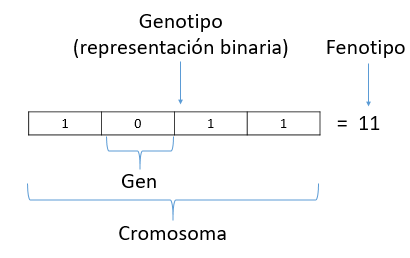
\includegraphics[width=0.75\linewidth]{img/fen_gen.png}
	\caption{Descripción grafica de genotipo, fenotipo, cromosoma y gen del numero ``11''}
	\label{fig:fen_gen}
\end{figure}

\subsection{Modelos generacionales y estacionarios}

En cada paso evolutivo, la cantidad de la población seleccionada y la forma de como se reintegran los nuevos individuos afectan el comportamiento general de la población, la velocidad en como evoluciona y el espacio de exploración para la búsqueda de óptimos globales.

Los \textbf{Modelos generacionales} actualizan la mayor parte de la población, se busca tener evoluciones rápida y una amplia exploración. Para ello se selecciona un pequeño conjunto de individuos y se les aplica los algoritmos de selección, cruza y mutación. Finalmente, mediante el algoritmo de reemplazo se reintegran en la población mediante una función.	

Por otro lado, los \textbf{modelos estacionarios} buscan mantener el equilibrio en la mayor parte de la población experimentando y mezclando un pequeño conjunto.  El cambio es mas lento pero mas estable.
	\chapter{Operador de Selección}

La función de selección elige las parejas (o subconjuntos) de individuos que fungirán como padres para reproducirse, combinar sus genes y generar la siguiente generación.

A continuación se presentan algunas funciones de selección, las cuales (en su mayoría) requieren los siguientes parámetros:
\begin{itemize}
	\item \texttt{population}: Subconjunto de la población al cual se le aplica el algoritmo.
	\item \texttt{objective}: Función de evaluación.
\end{itemize}

Algunas de las funciones son las siguientes:

\section{Universal Random}

La selección aleatoria universal (\textit{Universal Random}) es una variante estocástica de la selección proporcional que busca reducir la varianza introducida por la aleatoriedad. En lugar de seleccionar los individuos uno por uno, se generan múltiples puntos equidistantes sobre el intervalo $[0,1]$ para garantizar una muestra más representativa de la población, según sus probabilidades acumuladas.

Sea $n$ el número de individuos a seleccionar, se generan $n$ números equidistantes:
\[
r_i = \frac{i + u}{n} \quad \text{para } i = 0, 1, ..., n-1
\]
donde $u \sim U(0,1)$ es un número aleatorio uniformemente distribuido.

Cada número $r_i$ se mapea sobre la distribución acumulada de probabilidades para determinar a qué individuo seleccionar.

\begin{algorithm}[H]
	\caption{Universal Random Selection \\ \textbf{Input:} \{population, objective\}}
	\begin{algorithmic}[1]
		\State scores $\gets$ [objective($i$) for $i$ in population]
		\If{any score $<$ 0}
		\State scores $\gets$ scores - min(scores) \Comment{Normalización para evitar valores negativos}
		\EndIf
		\State total $\gets$ sum(scores)
		\State probabilities $\gets$ [score / total for score in scores]
		\State cumulative $\gets$ acumulada(probabilities)
		\State $u \gets$ random.uniform(0, 1)
		\For{$i = 0$ \textbf{to} population\_size}
		\State $r \gets \frac{i + u}{population\_size}$
		\State parents[$i$] $\gets$ individuo correspondiente a $r$ en la distribución acumulada
		\EndFor \\
		\Return parents
	\end{algorithmic}
	\label{alg:universal_random}
\end{algorithm}

Este método asegura una cobertura más uniforme de la población en comparación con la selección proporcional simple, reduciendo la varianza en la selección. Es particularmente útil cuando se desea mantener una representación proporcional sin depender completamente de la aleatoriedad individual de cada extracción.

\section{Tournament}

El algoritmo \ref{alg:tournament_selection} recibe, de manera adicional, el parámetro \texttt{selection\_rate}, que define el porcentaje de la población que participará en cada torneo.

Dada una población $P$, se selecciona aleatoriamente un subconjunto $Q \subseteq P$. El individuo $q_i$ con la mayor aptitud $f(q_i)$ es seleccionado para formar parte del conjunto de padres $S$:
\[
S = \left\{ \arg\max_{q \in Q} f(q) \,\middle|\, Q \subseteq P \right\}
\]

\begin{algorithm}[H]
	\caption{Tournament Selection \\ \textbf{Input:} \{population, objective, selection\_rate\}}
	\begin{algorithmic}[1]
		\For{$i = 0$ \textbf{to} population\_size}
		\State $k \gets$ population\_size $\times$ selection\_rate
		\State candidates $\gets$ random.sample(population, $k$)
		\State scores $\gets$ []
		\For{cada $j$ en candidates}
		\State scores.append(objective($j$))
		\EndFor
		\State max\_score $\gets$ max(scores)
		\State index $\gets$ scores.index(max\_score)
		\State parents[$i$] $\gets$ candidates[index]
		\EndFor \\
		\Return parents
	\end{algorithmic}
	\label{alg:tournament_selection}
\end{algorithm}

Este método es eficiente para poblaciones de cualquier tamaño. Además, el parámetro \texttt{selection\_rate} permite controlar la presión selectiva: torneos pequeños fomentan la diversidad, mientras que torneos grandes intensifican la explotación de los individuos más aptos.

\section{Proportional}

La selección proporcional (también conocida como \textit{roulette wheel selection}) asigna a cada individuo una probabilidad de ser seleccionado proporcional a su aptitud. Es un método estocástico que favorece a los individuos más aptos, pero permite la selección de individuos menos aptos con menor probabilidad, promoviendo así la diversidad.

Sea $P$ la población con $n$ individuos y $f(p_i)$ la función de aptitud del individuo $p_i$. La probabilidad de seleccionar al individuo $p_i$ se define como:

\[
\Pr(p_i) = \frac{f(p_i)}{\sum_{j=1}^{n} f(p_j)}
\]

\begin{algorithm}[H]
	\caption{Proportional Selection \\ \textbf{Input:} \{population, objective\}}
	\begin{algorithmic}[1]
		\State scores $\gets$ [objective($i$) for $i$ in population]
		\If{any score $<$ 0}
		\State scores $\gets$ scores - min(scores) \Comment{Normalización para evitar negativos}
		\EndIf
		\State total $\gets$ sum(scores)
		\State probabilities $\gets$ [score / total for score in scores]
		\State cumulative $\gets$ acumulada(probabilities)
		\For{$i = 0$ \textbf{to} population\_size}
		\State $r \gets$ random.uniform(0, 1)
		\State parents[$i$] $\gets$ individuo correspondiente a $r$ en la distribución acumulada
		\EndFor \\
		\Return parents
	\end{algorithmic}
	\label{alg:proportional_selection}
\end{algorithm}

Este método es intuitivo y funciona bien cuando las diferencias de aptitud entre individuos no son extremas. Sin embargo, si las diferencias son muy marcadas, puede provocar convergencia prematura. También es sensible a funciones de aptitud negativas o cercanas a cero, por lo que puede requerir normalización.

\section{Negative Assortative Mating}

El apareamiento negativo asortativo busca maximizar la diversidad genética al emparejar individuos que sean lo más diferentes posible entre sí. Este método es útil para evitar la convergencia prematura, ya que fomenta la exploración del espacio de soluciones.

Se utiliza una función de similitud $d(a, b)$ que cuantifica cuán parecidos son dos individuos $a$ y $b$. Esta función puede estar basada en distancia euclidiana, Hamming u otra métrica, según el tipo de representación del cromosoma. El objetivo es seleccionar, para cada individuo, una pareja que minimice dicha similitud.

\[
\text{Para cada } p_i \in P_{\text{seleccionado}},\quad p_j = \arg\min_{x \in P} \, d(p_i, x)
\]

\begin{algorithm}[H]
	\caption{Negative Assortative Mating \\ \textbf{Input:} \{population, similarity\_function\}}
	\begin{algorithmic}[1]
		\State num\_pairs $\gets$ population\_size / 2
		\State selected $\gets$ random.sample(population, num\_pairs)
		\State parents $\gets$ []
		\For{cada $p_i$ en selected}
		\State distances $\gets$ [similarity\_function($p_i$, $x$) for $x$ in population]
		\State eliminar $p_i$ de la población temporal para evitar emparejarlo consigo mismo
		\State partner $\gets$ individuo con menor valor de distancia
		\State parents.append(($p_i$, partner))
		\EndFor \\
		\Return parents
	\end{algorithmic}
	\label{alg:negative_assortative}
\end{algorithm}

Este método es particularmente útil en etapas tempranas del algoritmo evolutivo, donde la diversidad es crucial. Sin embargo, puede ser computacionalmente costoso, especialmente si se requiere calcular similitud entre todos los pares posibles en poblaciones grandes. Además, no garantiza que los individuos seleccionados sean de alta aptitud, por lo que suele combinarse con otros métodos de selección para mejorar su eficacia.

	\chapter{Operador de Cruza}

Los operadores de cruza permiten generar nuevos individuos (hijos) a partir de dos padres, combinando partes de sus cromosomas. A continuación se describen distintos métodos de cruza utilizados en algoritmos evolutivos.

\section{One Point}

Dados dos padres $p_1$ y $p_2$ con cromosomas de tamaño $T$, se selecciona una posición al azar $t \in [1, T-1]$ donde se particionan y combinan los genes:
\begin{gather*}
	h_1 = [0, t)_{p_1} \cup [t, T)_{p_2} \\
	h_2 = [0, t)_{p_2} \cup [t, T)_{p_1}
\end{gather*}

Tal como se muestra en la figura \ref{fig:cross_one}, con $t = 3$.

\begin{figure}[H]
	\centering
	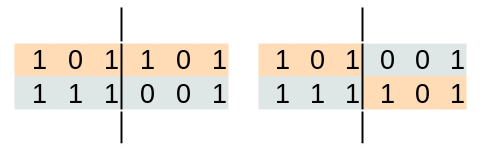
\includegraphics[width=0.75\linewidth]{img/cross_one.png}
	\caption{Ejemplo de cruza en un solo punto}
	\label{fig:cross_one}
\end{figure}

\section{Two Point}

Tiene un comportamiento similar al anterior. Dados dos padres $p_1$ y $p_2$ con cromosomas de tamaño $T$, se seleccionan dos posiciones al azar $t_1, t_2$ tales que $0 \leq t_1 < t_2 \leq T$. Se intercambia el segmento entre ambas posiciones:
\begin{gather*}
	h_1 = [0, t_1)_{p_1} \cup [t_1, t_2)_{p_2} \cup [t_2, T)_{p_1} \\
	h_2 = [0, t_1)_{p_2} \cup [t_1, t_2)_{p_1} \cup [t_2, T)_{p_2}
\end{gather*}

\begin{figure}[H]
	\centering
	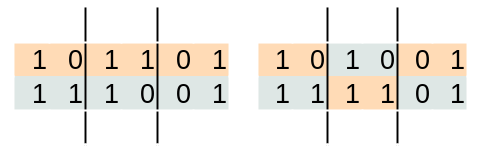
\includegraphics[width=0.75\linewidth]{img/cross_two.png}
	\caption{Ejemplo de cruza en dos puntos}
	\label{fig:cross_two}
\end{figure}

\section{Uniform}

Dados dos padres $p_1$ y $p_2$ con cromosomas de tamaño $T$, se genera una máscara binaria aleatoria $M \in \{0, 1\}^T$. Si $M[i] = 0$, entonces $h_1[i] = p_1[i]$ y $h_2[i] = p_2[i]$; si $M[i] = 1$, entonces $h_1[i] = p_2[i]$ y $h_2[i] = p_1[i]$.

\begin{figure}[H]
	\centering
	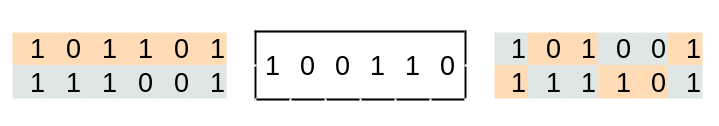
\includegraphics[width=0.75\linewidth]{img/cross_uniform.png}
	\caption{Ejemplo de cruza uniforme}
	\label{fig:cross_uniform}
\end{figure}

\section{Arithmetic}

Para cada par de padres, se genera un valor aleatorio $\alpha \in [0, 1]$ que define una combinación lineal entre sus genes. Para cada posición $i$ del cromosoma:
\begin{gather*}
	h_1[i] = \alpha \cdot p_1[i] + (1 - \alpha) \cdot p_2[i] \\
	h_2[i] = (1 - \alpha) \cdot p_1[i] + \alpha \cdot p_2[i]
\end{gather*}

Este operador es común en representaciones reales y mantiene los genes dentro del espacio de búsqueda.

\section{Blend (BLX-$\alpha$)}

El operador \textit{Blend Crossover} permite generar valores fuera del intervalo definido por los padres. Para cada gen $i$ se define un intervalo extendido:

\[
\text{min}_i = \min(p_1[i], p_2[i]), \quad
\text{max}_i = \max(p_1[i], p_2[i])
\]

El hijo se genera como:
\[
h[i] = U\left( \text{min}_i - d, \text{max}_i + d \right)
\quad \text{donde } d = \alpha \cdot (\text{max}_i - \text{min}_i)
\]

El parámetro $\alpha$ controla cuánto se puede explorar fuera del rango original. La función $U$ representa la distribución uniforme continua.

\section{Simulated Binary (SBX)}

El operador \textit{Simulated Binary Crossover} simula el comportamiento del cruce de un solo punto en cromosomas reales. Dado un parámetro de distribución $\eta$, se calcula un factor $\beta$ basado en una variable aleatoria $u \sim U(0,1)$:

\[
\beta = \begin{cases}
	(2u)^{1/(\eta + 1)} & \text{si } u \leq 0.5 \\
	\left( \frac{1}{2(1 - u)} \right)^{1/(\eta + 1)} & \text{si } u > 0.5
\end{cases}
\]

Entonces, los hijos se calculan como:
\begin{gather*}
	h_1[i] = 0.5 \cdot \left( (1 + \beta) \cdot p_1[i] + (1 - \beta) \cdot p_2[i] \right) \\
	h_2[i] = 0.5 \cdot \left( (1 - \beta) \cdot p_1[i] + (1 + \beta) \cdot p_2[i] \right)
\end{gather*}

\section{Uniform Order Based}

Este operador está diseñado para cromosomas con permutaciones (como en el problema del viajante). Se genera una máscara binaria $M$ de tamaño $T$. Las posiciones con 1 se copian directamente del primer padre al hijo. Las posiciones con 0 se rellenan, en orden, con los genes del segundo padre que no estén ya presentes en el hijo.

Este método mantiene la posición relativa y evita duplicados.

\section{Order Based}

También usado en permutaciones. Se seleccionan $k$ posiciones aleatorias del primer padre y se copian al hijo. Luego, se rellena el resto del hijo con los genes del segundo padre manteniendo el orden relativo y omitiendo duplicados.

Este operador es útil cuando el orden de los elementos en el cromosoma es relevante, como en rutas o secuencias.

\begin{table}[H]
	\centering
	\begin{tabular}{|l|c|c|}
		\hline
		\textbf{Operador de Cruza} & \textbf{Espacio que abarca} & \textbf{Representación}  \\ \hline
		One Point                  & Local                        & Binaria             \\ \hline
		Two Point                  & Local                        & Binaria             \\ \hline
		Uniform                    & Moderado                     & Binaria             \\ \hline
		Arithmetic                 & Local                        & Real                \\ \hline
		Blend (BLX-$\alpha$)       & Global (controlado por $\alpha$) & Real          \\ \hline
		Simulated Binary (SBX)     & Global (controlado por $\eta$)   & Real          \\ \hline
		Uniform Order Based        & Moderado                     & Permutacional       \\ \hline
		Order Based                & Moderado                     & Permutacional       \\ \hline
	\end{tabular}
	\caption{Comparativa de operadores de cruza según el tipo de representación y cobertura del espacio de búsqueda.}
	\label{tab:cross_comparison}
\end{table}

	\chapter{Operador de Mutación}

Una mutación es un cambio en el cromosoma que altera su valor; esta se aplica de forma independiente en cada individuo bajo cierta probabilidad $p$. La inclusión de mutaciones permite mantener la diversidad genética de la población y evita el estancamiento en óptimos locales cuando hay demasiada similitud entre individuos.

Dado que cada problema puede tener un espacio diferente (binario, reales, permutaciones), cada uno debe implementar una función que permita obtener un vecino aleatorio. Un vecino es una solución cercana a la actual, pero con una ligera variación. En este caso, la función \textit{Single Point} obtiene un vecino dada una solución actual, respetando la estructura del espacio de búsqueda.

\section{Single Point}

Este operador evalúa, para cada individuo en la población, si debe aplicarse una mutación basada en la probabilidad establecida. Si la condición se cumple, el individuo es reemplazado por un vecino generado por la función específica del problema; de lo contrario, permanece igual.

Este algoritmo permite mantener diversidad en la población sin alterar drásticamente la estructura de los individuos. Ademas, de que permite adaptarse a diferentes representaciones (binaria, real, permutaciones), aunque es fuertemente dependiente de la calidad de la función de \textit{getRandomNeighbour}.

\begin{algorithm}[H]
	\caption{Single Point Mutation \\ \textbf{Input} \{ population, problem, mutation\_rate \}}
	\begin{algorithmic}[1]
		\Function{SinglePoint}{population, problem, mutation\_rate}
		\State mutations $\gets$ [ ]
		\For{individual \textbf{in} population}
		\If{random() $\leq$ mutation\_rate}
		\State neighbor $\gets$ problem.getRandomNeighbour(individual)
		\State mutations.append(neighbor)
		\Else
		\State mutations.append(individual)
		\EndIf
		\EndFor
		\State \Return mutations
		\EndFunction
	\end{algorithmic}
	\label{alg:mutation_single}
\end{algorithm}


	\chapter{Operador de Reemplazo}

Este último operador se encarga de reintegrar la nueva población generada (producto de la selección, cruza y mutación) con la población actual. Su función es decidir quiénes sobreviven a la siguiente generación, balanceando la exploración del espacio de búsqueda con la preservación de soluciones prometedoras.

\section{Random}

Este enfoque selecciona aleatoriamente un subconjunto de la población actual para conservarlo y luego lo complementa con los nuevos individuos generados. No se considera la aptitud, lo que favorece la diversidad pero puede generar regresión en la calidad.

\begin{algorithm}[H]
	\caption{Random Replacement \\ \textbf{Input} \{ population, replace \}}
	\begin{algorithmic}[1]
		\Function{RandomReplace}{population, replace}
		\State $n \gets$ \texttt{len(population)}
		\State $k \gets$ \texttt{len(replace)}
		\State survivors $\gets$ \texttt{random.sample(population, n - k)}
		\State survivors $\gets$ survivors $+$ replace
		\State \Return survivors
		\EndFunction
	\end{algorithmic}
	\label{alg:replacement_random}
\end{algorithm}

Este algoritmo favorece la diversidad pero no garantiza la preservación de buenos individuos, porl o que puede perder soluciones óptimas.

\section{Elitism}

Este método conserva a los mejores individuos de la población actual, asegurando que las soluciones de alta calidad no se pierdan entre generaciones. Luego se complementa la población con los nuevos individuos generados.

\begin{algorithm}[H]
	\caption{Elitism Replacement \\ \textbf{Input} \{ population, replace, objective \}}
	\begin{algorithmic}[1]
		\Function{ElitismReplace}{population, replace, objective}
		\State $n \gets$ \texttt{len(population)}
		\State $k \gets$ \texttt{len(replace)}
		\State sorted\_pop $\gets$ \texttt{sorted(population, key=objective)}
		\State survivors $\gets$ sorted\_pop$[:n-k]$
		\State survivors $\gets$ survivors $+$ replace
		\State \Return survivors
		\EndFunction
	\end{algorithmic}
	\label{alg:replacement_elitism}
\end{algorithm}

A diferencia de \textit{random}, este si preserva los mejores individuos y acelera la convergencia hacia soluciones óptimas pero con riesgo de perder diversidad genética e incluso llevar a estancarlo en óptimos locales si se descuidan otros aspectos.

\section{Deterministic Crowding}

Este método busca mantener la diversidad genética mediante una competencia local entre padres e hijos similares. Cada hijo compite directamente con su padre más parecido (según una medida de distancia), y sobrevive el de mejor aptitud.

\begin{algorithm}[H]
	\caption{Deterministic Crowding Replacement \\ \textbf{Input} \{ parents, offspring, objective, distance \}}
	\begin{algorithmic}[1]
		\Function{DeterministicCrowding}{parents, offspring, objective, distance}
		\State survivors $\gets$ [ ]
		\For{$i = 0$ \textbf{to} len(parents) step 2}
		\State $p_1, p_2 \gets$ parents[i], parents[i+1]
		\State $o_1, o_2 \gets$ offspring[i], offspring[i+1]
		
		\If{distance($p_1$, $o_1$) + distance($p_2$, $o_2$) < distance($p_1$, $o_2$) + distance($p_2$, $o_1$)}
		\State winners $\gets$ [ \texttt{argmax}($p_1$, $o_1$), \texttt{argmax}($p_2$, $o_2$) ]
		\Else
		\State winners $\gets$ [ \texttt{argmax}($p_1$, $o_2$), \texttt{argmax}($p_2$, $o_1$) ]
		\EndIf
		\State survivors.extend(winners)
		\EndFor
		\State \Return survivors
		\EndFunction
	\end{algorithmic}
	\label{alg:replacement_deterministic_crowding}
\end{algorithm}

Mantiene la diversidad poblacional y favorece la exploración de nichos a cambio de poder computacional.

\section{Restricted Tournament Selection (RTS)}

Este método también promueve la diversidad al restringir las competencias a individuos similares. Cada hijo compite contra un subconjunto aleatorio de la población, y se reemplaza al más parecido si el hijo tiene mejor aptitud.

\begin{algorithm}[H]
	\caption{Restricted Tournament Selection \\ \textbf{Input} \{ population, offspring, objective, window\_size, distance \}}
	\begin{algorithmic}[1]
		\Function{RTS}{population, offspring, objective, window\_size, distance}
		\For{child in offspring}
		\State window $\gets$ random.sample(population, window\_size)
		\State closest $\gets$ \texttt{argmin}(\texttt{[distance(child, w) for w in window]})
		\If{objective(child) > objective(closest)}
		\State population[population.index(closest)] $\gets$ child
		\EndIf
		\EndFor
		\State \Return population
		\EndFunction
	\end{algorithmic}
	\label{alg:replacement_rts}
\end{algorithm}

Mantiene estructuras locales de la población pero depende del calculo de distancias, lo que puede ser costoso.
	\chapter{Problemas}

\section{Knapsack problem}

Dado un conjunto de $n$ ítems \[I = \{1,2, \dots, n \}\] Donde cada ítem $i$ tiene un valor $v_i \geq 0$ y un peso $w_i \geq 0$ y dada una mochila con capacidad máxima $W$, se busca seleccionar un subconjunto de ítems que maximice el valor total sin exceder la capacidad.

Podemos representar los elementos dentro de la mochila como un vector binario: 
\[ x = (x_1, x_2, \dots , x_n) \; \text{con } x_i \in \{0, 1\} \]
Donde:
\begin{itemize}
	\item $x_i = 0$ si el ítem no esta en la mochila
	\item $x_i = 1$ si el ítem si esta en la mochila
\end{itemize}

Para calcular el valor $v(x)$ y el peso $w(x)$ de la mochila sumamos los valores que si se encuentren dentro de ella:
\begin{gather*}
	v(x) = \sum_{i = 1}^{n} v_i x_i \\
	w(x) = \sum_{i = 1}^{n} w_i x_i 
\end{gather*}

El objetivo, es encontrar el mayor $v(x)$ siempre que el peso $w(x)$ no exceda el peso máximo $W$. 

\begin{itemize}
	\item El conjunto de estados posibles son todas las cadenas binarias de tamaño $n$: \[ S = \{ x \in \{ 0, 1  \}^n \} \]
	
	\item El estado inicial puede ser cualquier cadena de tamaño $n$ cuyo peso no exceda el peso máximo: \[ s_0 = \{x \in \{0,1\}^n | w(x) \leq W \} \]
	
	\item Se busca maximizar el valor de la mochila. La función objetivo suma los valores de los objetos dentro de la mochila. Si el peso de la mochila excede el limite, entonces se le asigna una ganancia negativa. 
	\[
	f(x) =
	\begin{cases} 
		v(x), & \text{si } w(x) \leq W \\ 
		W - w(x), & \text{si } w(x) > W
	\end{cases}
	\]
	
	Se le asigna la diferencia del peso máximo menos el peso actual (Dando un numero negativo). Esto con el objetivo de que, si por alguna razón esa es la mejor solución actual, sepa encontrar una mejor solución disminuyendo esa diferencia.
	
	\item Entonces, un estado $x_j$ es un estado final si genera mayor aptitud en comparación de los demás $x_i$ generados y tiene una aptitud no negativa: \[ f(x_j) \geq 0 \land f(x_j) \geq f(x_i) \; \forall x_i \in S\]
	
	\item La operación que genere genere el vecino sera \textit{Bit flip} que intercambia un 0 por un 1 y viceversa en una posición aleatoria $i$).
	
	\[
	B(x_i) =
	\begin{cases} 
		1, & \text{si } x_i = 0 \\ 
		0, & \text{si } x_i = 1 \\
	\end{cases}
	\]
	
\end{itemize}

\section{Travel Salesman Problem (TSP)}

Dado un conjunto de $n$ ciudades \[ C = \{1,2, \dots , n\} \] Y una matriz simétrica $M$ que almacena las distancias entre las ciudades, se busca encontrar el camino hamiltoniano con menor distancia a recorrer. Es decir, se busca encontrar el recorrido de ciudades con la menor distancia pasando solo una vez por ciudad y regresando a la primera.

Podemos representar la trayectoria de las ciudades como un vector de enteros:
\[ x = (x_1, x_2, \dots, x_n) \; \text{con } x_i \in [1, n] \]
Donde:
\begin{itemize}
	\item $x_i = c$ es la ciudad $c$ visitada en la i-ésima posición. Es necesario que cada $c$ sea único en cada ruta $x$, es decir, que $x$ sea una permutación de $C$.
\end{itemize}

Para calcular la distancia, iteramos el vector en orden y consultamos las distancias de cada par en la matriz $M$: 
\[ d(x) = \sum_{i = 1}^{n} M(x_i, x_{i \%(n+1)+ 1}) \]

El objetivo, es encontrar la ruta $x$ que minimice la distancia $d(x)$ siempre que la ruta no tenga ciudades $c$ repetidas.

\begin{itemize}
	\item El conjunto de estados posibles son todas las cadenas de enteros de tamaño $n$ que sean una permutación de $C$: \[ S = \{ x \in [1, n]^n \;|\; x \text{ es una permutación de } C \} \]
	
	\item El estado inicial puede ser cualquier permutación de $C$: 
	\[ s_0 = \{ x \in [1, n]^n \;|\; x \text{ es una permutación de } C \} \]
	
	\item Se busca minimizar la ruta. La función objetivo suma todas las distancias de la ruta planeada. Si una ciudad se visita mas de una vez, entonces se le asigna una ganancia nula. Dado que queremos minimizar la función, se le asigna infinito.
	\[
	f(x) =
	\begin{cases} 
		d(x), & \text{si } \forall c \in C \colon \{ c \in x \} \\ 
		\infty, & \text{si } \exists c \in C \colon \{c \notin x\}
	\end{cases}
	\]
	Esto significa que:
	\begin{itemize}
		\item Se le asigna $d(x)$ si todas las ciudades se encuentran en la ruta. Dado que la ruta es del mismo tamaño que el numero de ciudades, si aparecen todas las ciudades, entonces no hay ciudades repetidas.
		\item Se le asigna $\infty$ si existe una ciudad que no aparezca en la ruta. Si una ciudad no aparece en la ruta, significa que al menos una ciudad aparece dos veces, por lo que se repite.
	\end{itemize}
	
	\item Entonces, un estado $x_j$ es un estado final si genera una menor aptitud en la comparación de los demás $x_i$ generados: \[ f(x_j) \leq f(x_i) \; \forall x_i \in S \]
	
	\item La operación que genere los vecinos sera \textit{Swap}, ya que asegura unicamente cambiar el orden de los elementos sin tener que repetir ciudades. Esto implica que: \[ x_i = x_j \; \&  \; x_j = x_i \]
	
\end{itemize}



Nótese que el estado inicial puede ser un estado de aceptación. Si realizamos puras operaciones \textit{Swap}, no estamos añadiendo ni quitando ciudades, sino que unicamente se obtiene una nueva permutación. Por lo que podemos redefinir la función objetivo como: \[ f(x) = d(x) \] Y el conjunto de estados posibles como cualquier vector de tamaño $n$ que tenga números únicos en rango de $[1,n]$: \[ S = \{ x \in \{1, 2, \dots, n  \}^n | \forall x_i \colon \forall x_j \colon x_i \neq x_j \}\]

\section{Minimizar la función}

Obtener los mínimos de la función \[ f(x) = \ \sum_{i = 1}^{D} x_i^2, \; \text{ con } -10 \geq x_i \geq 10 \].

Dado un vector de $D$ números en el rango de $[-10, 10]$, se busca obtener el valor mínimo del sumatoria  de sus cuadrados.

\begin{itemize}
	\item El conjunto de estados posibles son todas las cadenas de enteros en dicho intervalo: \[ S = \{ x \in [-10, 10]^n \} \]
	
	\item El estado inicial se genera de forma arbitraria como un vector de $D$ números en el rango establecido $[-10, 10]$
	
	\item La función objetivo unicamente considera los valores dentro del propio vector: \[f(x) \]
	
	\item Un estado de aceptación $x_j$ es aquel que produzca el menor valor de aptitud en la función comparando con los demás $x_i$ generados: \[ f(x_j) \leq f(x_i) \; \forall x_i \in S\] 
	
	\item La operación que genere los vecinos puede tener multiples interpretaciones. Para este problema se asume un espacio circular donde $-10$ es el consecutivo del $10$ y que $\forall d_i \in D, d_i \in \mathbb{Z}$.  Entonces, los vecinos de $d_i$ son los números consecutivos, es decir $d_{i-1}$ y $d_{i+1}$.
	
	La operación sera entonces:
	\[ d_i = min(f(d_{i-1}), f(d_i), f(d_{i+1})) \]	
\end{itemize}

\clearpage
\section{Problemas de optimización CEC 2017}

En el documento \cite{cec} se presentan una serie de problemas sobre optimización numérica de parámetros reales. En este reporte se analizan las 10 primeras funciones que cumplen con la siguiente definición:
\begin{itemize}
	\item Todas las funciones son problemas de minimización definidos de la siguiente manera:
	\[ min f(x), \; x = [x_1, x_2, \dots, x_D]^T \]
	Donde:
	\begin{itemize}
		\item $x$ es el vector de variables de dimensión $D$ que representa la solución del problema.
		\item $D$ es el numero de dimensiones del problema.
	\end{itemize}
	
	\item El óptimo global (la mejor solución) se encuentra desplazada del origen para evitar respuestas que asumen que la respuesta esta cerca del origen:
	\[ o = [ o_1, o_2, \dots, o_D ]^T \]
	Donde $o$ es el vector del optimo global desplazado.
	
	El valor óptimo se distribuye de manera aleatoria en el rango de $o \in [-80, 80]^D$
	
	\item Las funciones son escalables, es decir, el numero de dimensiones $D$ puede variar.
	
	\item El rango de búsqueda de todas las funciones para las variables se delimita por $x \in [-100, 100]^D$
	
	\item Implementación de matrices de rotación: Las variables interactúan entre ellas para volver el problema más difícil.
	
	\item Para simular problemas reales, las variables se dividen de manera aleatoria en subcomponentes. Cada subcomponente tiene su propia matriz de rotación.
	
\end{itemize}

\subsection{Funciones}

A continuación se definen las 10 primeras funciones.

\subsubsection*{1) Bent Cigar Function}
\[
f(x) = x_1^2 + 10^6 \sum_{i=2}^{D} x_i^2
\]

\subsubsection*{2) Zakharov Function}
\[
f(x) = \sum_{i=1}^{D} x_i^2 + \left( 0.5 \sum_{i=1}^{D} i x_i \right)^2 + \left( 0.5 \sum_{i=1}^{D} i x_i \right)^4
\]

\subsubsection*{3) Rosenbrock's Function}
\[
f(x) = \sum_{i=1}^{D-1} \left[ 100 (x_{i+1} - x_i^2)^2 + (x_i - 1)^2 \right]
\]

\subsubsection*{4) Rastrigin's Function}
\[
f(x) = \sum_{i=1}^{D} \left[ x_i^2 - 10 \cos(2 \pi x_i) + 10 \right]
\]

\subsubsection*{5) Expanded Schaffer's F6 Function}
\[
g(x, y) = 0.5 + \frac{\sin^2(\sqrt{x^2 + y^2}) - 0.5}{(1 + 0.001(x^2 + y^2))^2}
\]

\[
f(x) = \sum_{i=1}^{D-1} g(x_i, x_{i+1})
\]

\subsubsection*{6) Lunacek Bi-Rastrigin Function}
\[
f(x) = \min \left( \sum_{i=1}^{D} (x_i - \mu_0)^2, dD + s \sum_{i=1}^{D} (x_i - \mu_1)^2 \right) 
+ 10 \sum_{i=1}^{D} \left[ 1 - \cos(2 \pi z_i) \right]
\]

\[
\mu_0 = 2.5, \quad \mu_1 = -\sqrt{\frac{\mu_0^2}{d}}
\]

\subsubsection*{7) Non-Continuous Rotated Rastrigin's Function}
\[
f(x) = \sum_{i=1}^{D} \left[ z_i^2 - 10\cos(2\pi z_i) + 10 \right]
\]

\[
z_i = \text{Tosz}(\text{Tasy}(x_i))
\]

\subsubsection*{8) Levy Function}
\[
f(x) = \sin^2(\pi w_1) + \sum_{i=1}^{D-1} (w_i - 1)^2 \left[ 1 + 10\sin^2(\pi w_i + 1) \right] + (w_D - 1)^2 \left[ 1 + \sin^2(2\pi w_D) \right]
\]

\[
w_i = 1 + \frac{x_i - 1}{4}
\]

\subsubsection*{9) Modified Schwefel's Function}
\[
f(x) = 418.9829 D - \sum_{i=1}^{D} x_i \sin(\sqrt{|x_i|})
\]

\subsubsection*{10) High Conditioned Elliptic Function}
\[
f(x) = \sum_{i=1}^{D} 10^{6 \frac{i-1}{D-1}} x_i^2
\]

Cuyas graficas se observan en la figura \ref{fig:cec}

\begin{figure}[H]
	\centering
	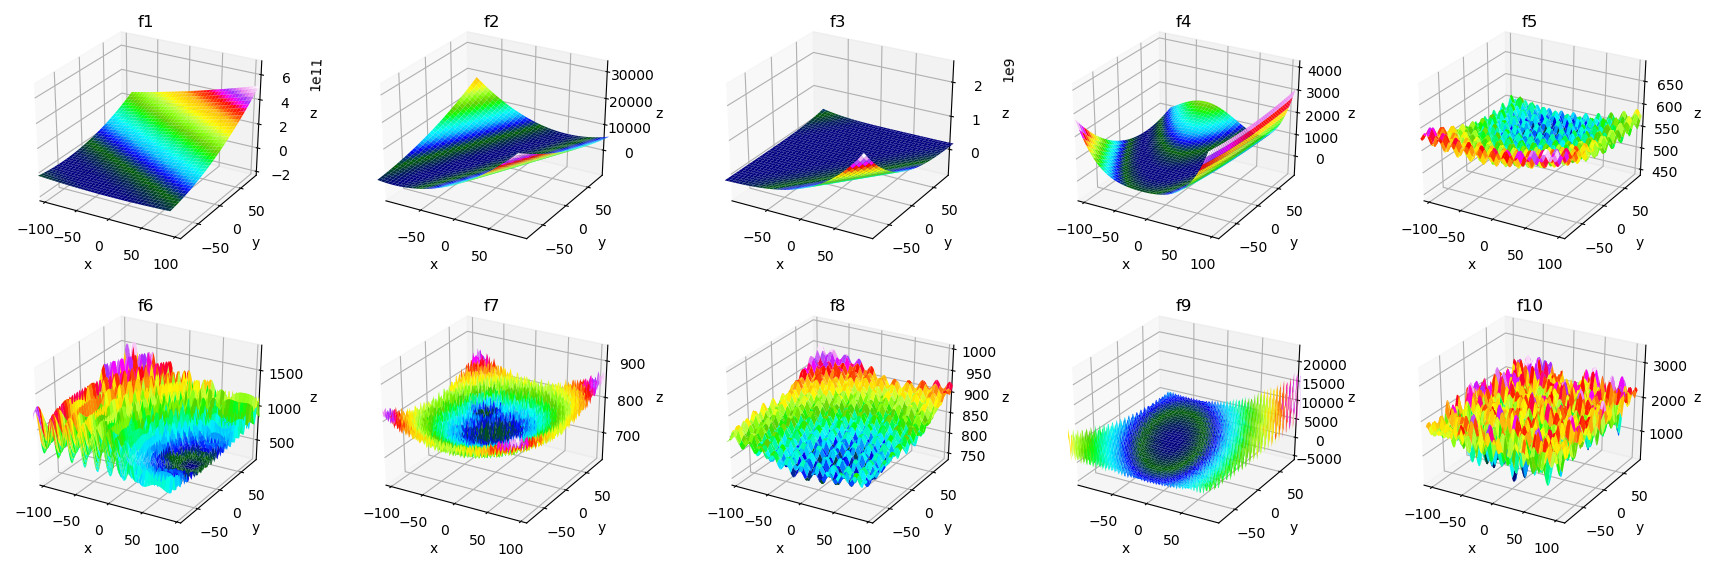
\includegraphics[width=1\linewidth]{img/cec}
	\caption{Superficies ploteadas de las 10 primeras funciones para dos dimensiones \cite{plot}}
	\label{fig:cec}
\end{figure}
	\chapter{Codigo}

\section{Problem}

Los problemas a optimizar siguen una mista estructura. Dado esto, se optó por diseñar una clase que generaliza el problema y permite y facilita la definición de nuevos problemas.

El código \ref{lst:problem} incluye los siguientes métodos los cuales deben de ser implementados por sus clases hijas:
\begin{itemize}
	\item \textit{generateInformation}: Función que define la información necesaria para calcular la función objetivo. La información adicional depende del problema.
	\item \textit{objective}: Función que calcula la utilidad de la solución, si es un problema de minimización tiene que devolver con el signo opuesto. 
	\item \textit{generateInitialSolution}: Función que genera una solución.
	\item \textit{getRandomNeighbour}: Obtiene un vecino de forma aleatoria.
	\item \textit{getNextNeighbour}: Si es necesario manejar indices, esta función permite obtener un vecino tras otro.
	\item \textit{getNeighbours}: Devuelve todos los vecinos.
\end{itemize}

\begin{lstlisting}[style=pythonstyle, label={lst:problem} ,caption={Clase \textit{problem}}]
class Problem(ABC):
  def __init__(self,):
  self.information:Any = {}

  @abstractmethod
  def generateInformation(self, *args, **kwargs) -> None: pass

  @abstractmethod
  def objective(self, solution: Any) -> float: pass

  @abstractmethod
  def generateInitialSolution(self) -> Any: pass

  @abstractmethod
  def getRandomNeighbour(self, solution:Any) -> Any: pass

  @abstractmethod
  def getNextNeighbour(self, solution:Any, *args, **kwargs) -> Any: pass

  @abstractmethod
  def getNeighbours(self, solution: Any) -> list: pass

  @abstractmethod
  def printInformation(self) -> None: pass
\end{lstlisting}

\subsubsection{Knapsack problem}

La clase \textit{knapsackProblem} hereda de la clase \textit{Problem} e implementa las siguientes funciones.

La función \ref{lst:kp-gi} genera de manera aleatoria un conjunto de elementos en la mochila con pesos y valores aleatorios en un rango de $[1,10]$. La función \ref{lst:kp-e} calcula la energía del sistema la cual suma todos los pesos y valores de los elementos que se encuentran en la solución, si el peso es menor al capacidad de la mochila entonces devuelve el valor de la mochila, en caso contrario devuelve la diferencia de el peso actual menos la capacidad máxima.

La función \ref{lst:kp-gis} genera soluciones aleatorias de combinaciones y no regresa ninguna de ellas hasta que el peso de la solución sea menor a la capacidad máxima. Finalmente, la función \ref{lst:kp-rn} se encarga de generar un vecino de forma aleatoria, primero selecciona un elemento aleatorio del vector y después lo invierte.  

\begin{lstlisting}[style=pythonstyle, label={lst:kp-gi} ,caption={Función \textit{generateInformation} de Knapsack problem}]
def generate_information(self, items, capacity):
  self.information = {
	"items": items,
	"values": [(random.randint(1,10), random.randint(1, 10)) for _ in range(items)],
	"capacity": capacity
  }
\end{lstlisting}

\begin{lstlisting}[style=pythonstyle, label={lst:kp-e} ,caption={Función \textit{objective} de Knapsack problem}]
def objective(self, solution):
  total_weight = total_value = 0
  for i, selected in enumerate(solution):
    if selected:
      total_weight += self.information["values"][i][0]
  	  total_value += self.information["values"][i][1]
  if total_weight > self.information["capacity"]:
    return self.information["capacity"] - total_weight 
  return total_value
\end{lstlisting}

\begin{lstlisting}[style=pythonstyle, label={lst:kp-gis} ,caption={Función \textit{generateInitialSolution} de Knapsack problem}]
def generateInitialSolution(self):
  return [random.randint(0, 1) for _ in self.information['values']]
\end{lstlisting}

\begin{lstlisting}[style=pythonstyle, label={lst:kp-rn} ,caption={Función \textit{getRandomNeighbour} de Knapsack problem}]
def getRandomNeighbour(self, solution):
  neighbour = solution[:]
  index = random.randint(0, len(solution) - 1)
  neighbour[index] = 1 - int(neighbour[index])
  return neighbour  
\end{lstlisting}

Para el algoritmo genético, no es necesario especificar el resto de funciones.

\subsection{Travel Salesman Problem}

La función \ref{lst:tsp-gi} genera una matriz cuadrada y simétrica de $n$ valores aleatorios en un rango de $[1, 100]$.

La función \ref{lst:tsp-e} calcula la energía del sistema. Dado un vector suma todas las distancias de las ciudades con base en la información generada en \ref{lst:tsp-gi}, el resultado que devuelve es negativo ya que se busca minimizar. La función \ref{lst:tsp-gis} genera un vector de $n$ números consecutivos (representando las ciudades) y cambia las posiciones mediante la función \textit{shuffle}.

Finalmente, la función \ref{lst:tsp-rn} toma dos indices aleatorios diferentes e invierte los valores de dichas posiciones del vector.

\begin{lstlisting}[style=pythonstyle, label={lst:tsp-gi} ,caption={Función \textit{generateInformation} de Travel Salesman Problem}]
def generateInformation(self, cities: int):
  distances = [[0]*cities for _ in range(cities)]

  for i in range(cities):
    for j in range(i, cities):  
      if i == j:
        valor = 0  
      else:
        valor = random.randint(1, 100)
      distances[i][j] = valor
  	  distances[j][i] = valor 

  self.information = {
	"cities" : cities,
	"distances" : distances
  }
\end{lstlisting}

\begin{lstlisting}[style=pythonstyle, label={lst:tsp-e} ,caption={Función \textit{Objective} de Travel Salesman Problem }]
def objective(self, solution):
  distance = 0
  num_cities:int = len(solution)

  for i in range(num_cities):
    current_city = solution[i]
    next_city = solution[(i + 1) % num_cities]  
    distance += self.information['distances'][current_city][next_city]

  return -distance
\end{lstlisting}

\begin{lstlisting}[style=pythonstyle, label={lst:tsp-gis} ,caption={Función \textit{generateInitialSolution} de Travel Salesman Problem}]
def generateInitialSolution(self):
  solution =  list(range(self.information['cities']))
  random.shuffle(solution)
  return solution   
\end{lstlisting}

\begin{lstlisting}[style=pythonstyle, label={lst:tsp-rn} ,caption={Función \textit{getRandomNeighbour} de Travel Salesman Problem}]
def getRandomNeighbour(self, solution):
  neighbour = solution[:]
  i = j = random.randint(0, len(solution) - 1)
  while j == i:
    j = random.randint(0, len(solution) - 1)
  neighbour[i], neighbour[j] = neighbour[j], neighbour[i]

  return neighbour
\end{lstlisting}

\subsection{Sum function Problem}

La función \ref{lst:sfp-gi} unicamente define el tamaño del vector y los rangos de valores. por otro lado, la función \ref{lst:sfp-e} calcula la energía del sistema dada por la suma de los cuadrados, dado que es una función de minimización se invierte el signo.

La función \ref{lst:sfp-gis} genera un vector de $n$ elementos aleatorios en los rangos definidos, mientras que la función \ref{lst:sfp-gn} suma  o resta en uno a un elemento aleatorio del vector (dado que se considera una configuración circular, se ajusta el valor si el nuevo valor no se encuentra en el rango).

\begin{lstlisting}[style=pythonstyle, label={lst:sfp-gi} ,caption={Función \textit{generateInformation} de SumFunctionProblem}]
def generateInformation(self, size: int, min: int, max: int):
  self.information = {
	"size": size,
	"min": min,
	"max": max
  }
\end{lstlisting}

\begin{lstlisting}[style=pythonstyle, label={lst:sfp-e} ,caption={Función \textit{objective} de SumFunctionProblem}]
def objective(self, solution):
  total_sum:float = 0

  for val in solution:
    total_sum += val**2

  return -total_sum
\end{lstlisting}

\begin{lstlisting}[style=pythonstyle, label={lst:sfp-gis} ,caption={Función \textit{generateInitialSolution} de SumFunctionProblem}]
def generateInitialSolution(self):
  solution = [random.randint(self.information['min'], self.information['max']) for _ in range(self.information['size'])]
  return solution
\end{lstlisting}

\begin{lstlisting}[style=pythonstyle, label={lst:sfp-gn} ,caption={Función \textit{getRandomNeighbour} de CEC 2017}]
def getRandomNeighbour(self, solution):
  neighbour = solution[:]
  index = random.randint(0, len(solution) - 1)
  sign = random.choice([-1 , 1])
  neighbour[index] += sign

  if neighbour[index] > self.information['max']:
    neighbour[index] = self.information['min']

  if neighbour[index] < self.information['min']:
	neighbour[index] = self.information['max']

  return neighbour
\end{lstlisting}

\subsection{CEC 2017}

La función \ref{lst:cec-gi} define la función a optimizar, los rangos de valores, el tamaño de la dimensión y la tasa de cambio (ya que la solución es real). Por otro lado, la función \ref{lst:cec-e} calcula la energía del sistema dados los parámetros ya definidos.

La función \ref{lst:cec-gis} genera un vector de la dimensión definida restringida por la información adicional definida, mientras que la función \ref{lst:cec-gn} suma  o resta en \textit{alpha} a un elemento aleatorio del vector.

\begin{lstlisting}[style=pythonstyle, label={lst:cec-gi} ,caption={Función \textit{generateInformation} de CEC 2017}]
def generateInformation(self, function: callable, low:int, high:int, dimention:int, alpha:int):
  self.information = {
	"function": function,
	"low" : low,
	"high": high,
	"dimention": dimention,
	"alpha": alpha
  }
\end{lstlisting}

\begin{lstlisting}[style=pythonstyle, label={lst:cec-e} ,caption={Función \textit{objective} de CEC 2017}]
def objective(self, solution):
  return - self.information["function"]([solution])[0]
\end{lstlisting}

\begin{lstlisting}[style=pythonstyle, label={lst:cec-gis} ,caption={Función \textit{generateInitialSolution} de CEC 2017}]
def generateInitialSolution(self):
  solution = np.random.uniform(low=self.information["low"],
    high=self.information["high"],
    size=self.information["dimention"]).tolist()

  return solution
\end{lstlisting}

\begin{lstlisting}[style=pythonstyle, label={lst:cec-gn} ,caption={Función \textit{getRandomNeighbour} de CEC 2017}]
def getRandomNeighbour(self, solution):
  neighbour = solution[:]
  index = random.randint(0, len(solution) - 1)
  alpha = random.uniform(-self.information["alpha"], self.information["alpha"])

  neighbour[index] += alpha
  return neighbour
\end{lstlisting}

\section{Metaheuristic}

De igual manera, el se diseña una clase padre \ref{lst:meta} que implemente algunas de las funciones compatibles entre algoritmo genético, \textit{hill climbing} y \textit{simulated annealing}.

Esta clase tiene como parametro la clase \textit{Problem} y define los métodos abstractos \textit{resetProblem} y \textit{optimize} los cuales reinician meta parámetros y evalúan el algoritmo, respectivamente.

Adicionalmente se definen 3 funciones:
\begin{itemize}
	\item \textit{evaluate}: recibe como parámetro una solución y devuelve la aptitud definida por el problema
	
	\item \textit{isBetterSolution}: Compara dos soluciones.
	
	\item \textit{isSameSolution}: Verifica si dos soluciones tiene  la misma aptitud.
\end{itemize}

\begin{lstlisting}[style=pythonstyle, label={lst:meta} ,caption={Clase \textit{Metaheuristic}}]
class Metaheuristic(ABC):
  def __init__(self, problem: Problem):
  self.problem = problem

  @abstractmethod
  def resetProblem(self):
    self.solution = self.problem.generateInitialSolution()
    self.is_best = False

  @abstractmethod
  def optimize(self, *args, **kwargs): pass

  def evaluate(self, state: Any) -> float:
    return self.problem.objective(state)

  def isBetterSolution(self, solution_1: Any, solution_2: Any)-> bool:
    return (self.problem.objective(solution_1) > 
    	self.problem.objective(solution_2)) 

  def isSameSolution(self, solution_1: Any, solution_2: Any) -> bool:
  return (self.problem.objective(solution_1) ==
  	  self.problem.objective(solution_2)) 

  def printSolution(self) -> None:
    print(f'Solution: {self.solution}: {self.evaluate(self.solution)}')

  def getSolution(self) -> Any:
    return self.solution

  def setSolution(self, solution: Any):
    self.solution = solution
\end{lstlisting}

\subsection{Genetic Algorithm}

La clase \textit{GeneticAlgorithm} hereda de la clase \textit{Metaheuristic} e incluye las clases \textit{GASelectionFunctions}, \textit{GACrossoverFunctions}, \textit{GAMutationFunctions} y \textit{GAReplaceFunctions} que se verán mas adelante.

El constructor del código \ref{lst:ga-init} recibe como parametros el problema de optimización y el tamaño de la población. Adicionalmente crea los objetos de las funciones para poder ser accedidas desde esa misma clase y llama la función \ref{lst:ga-rp}, la cual predefine las funciones del algoritmo e inicializa la población.

La función \ref{lst:ga-o} se encarga de encontrar la mejor solución realizando las operaciones de selección, cruza, mutación y reemplazo. Nótese que esta función recibe como parámetro \textit{stationary} de tipo \textit{float} el cual define el tamaño de la población que se mantiene estacionaria y cual evoluciona. A la parte que evoluciona se le aplican las operaciones de selección, cruza y mutación para al final aplicar la operación de reemplazo a la población en general.

Adicionalmente, la función \ref{lst:ga-set} es el \textit{setter} de la función a utilizar, el resto de funciones tienen la misma estructura. Se utiliza \textit{partial} ya que existen funciones que requieren de parámetros adicionales.

\begin{lstlisting}[style=pythonstyle, label={lst:ga-init} ,caption={Constructor  \textit{GeneticAlgorithm}}]
	class Metaheuristic(ABC):
def __init__(self, problem, population_size: int = 16):
  super().__init__(problem)
  self.population_size = population_size
  self.selection_functions = Selection
  self.crossover_functions = Crossover
  self.mutation_functions = Mutation
  self.replace_functions = Replace
  self.resetProblem()
\end{lstlisting}

\begin{lstlisting}[style=pythonstyle, label={lst:ga-rp} ,caption={Función  \textit{resetProblem}}]
def resetProblem(self):
super().resetProblem()
self.population = [self.problem.generateInitialSolution() for _ in range(self.population_size)]
self.selection = Selection.tournament
self.crossover = Crossover.onePoint
self.mutation = Mutation.singlePoint
self.replace = Replace.random
\end{lstlisting}

\begin{lstlisting}[style=pythonstyle, label={lst:ga-o} ,caption={Función  \textit{optimize}}]
def optimize(self, epochs: int = 1, stationary: float = 0):
  for _ in range(epochs):
    population_sample = random.sample(self.population,self.population_size - int(self.population_size * stationary))

    population_sample = self.selection(population_sample, self.problem.objective)
    population_sample = self.crossover(population_sample)
    population_sample = self.mutation(population_sample, self.problem)
    self.population = self.replace(self.population, population_sample, self.problem.objective) 
\end{lstlisting}

\begin{lstlisting}[style=pythonstyle, label={lst:ga-set} ,caption={Función  \textit{optimize}}]
def setSelection(self, selection, selection_rate = None):
  if selection_rate:
    self.selection = partial(selection, selection_rate = selection_rate)
  else:
    self.selection = selection
\end{lstlisting}

\subsection{Selection functions}

Las funciones de selección reciben como parametros la población de la cual se seleccionan los padres, la función objetivo y retorna el conjunto de individuos de padres de la siguiente generación.

 A conitnuación se muestran tres operadores de selección: 
 \begin{itemize}
 	\item \textit{tournament}. Recibe un parámetro adicional que define la cantidad de individuos que participaran en cada torneo.
 	\item \textit{proportional}
 	\item \textit{negativeAssortativeMating}. Aunque recibe como parámetro la función objetivo no es requerida, ya que es at función busca emparejar aquellos individuos mas diferentes.
 \end{itemize}
 
\begin{lstlisting}[style=pythonstyle, label={lst:ga-t} ,caption={Función  \textit{tournament}}]
@staticmethod
def tournament(population, objective, selection_rate=0.2):
  population_size = len(population)
  parents = []

  for _ in range(population_size):
    k = max(2, math.ceil(population_size * selection_rate))
    candidates = random.sample(population, min(k, population_size))
    scores = [objective(ind) for ind in candidates]
    best = candidates[scores.index(max(scores))]
    parents.append(best)

  return parents    
\end{lstlisting}

\begin{lstlisting}[style=pythonstyle, label={lst:ga-p} ,caption={Función  \textit{proportional}}]
@staticmethod
def proportional(population, objective):
  population_size = len(population)
  parents = []

  objectives = SelectionFunctions._linealDisplacement(population, objective)

  total = sum(objectives)
  probabilities = [ objective/total for objective in objectives ]

  proportions = [ probabilities[0] ]
  for i in range(1, len(probabilities)):
    proportions.append(probabilities[i] + proportions[i - 1])

  for _ in range(population_size):
    pos = random.random()
    for i in range(len(proportions)):
      if (pos <= proportions[i]):
        parents.append(population[i])
        break

  return parents
\end{lstlisting}

\begin{lstlisting}[style=pythonstyle, label={lst:ga-nam} ,caption={Función  \textit{negativeAssortativeMating}}]
@staticmethod
def negativeAssortativeMating(population, objective):
  population_size = len(population)
  parents = []

  for _ in range(int(population_size/2)):
    individual = random.choice(population)
    distances = [ SelectionFunctions.distance(individual, test) for test in population ]

    parents.append(individual)
    parents.append(population[distances.index(max(distances))])

  return parents
\end{lstlisting}

\subsection{Crossover functions}

A continuación, se muestra la implementación de tres algoritmos de cruza:
\begin{itemize}
	\item \textit{onePoint} para soluciones binarias.
	\item \textit{arithmetic} para soluciones reales.
	\item \textit{uniformOrderBased} para soluciones de permutación.
\end{itemize}

\begin{lstlisting}[style=pythonstyle, label={lst:ga-op} ,caption={Función  \textit{onePoint}}]
def onePoint(population:list):
  generation:list = []    
  population_size = len(population)
  for i in range(0, population_size, 2):
    parent1 = population[i]
    parent2 = population[i + 1]

    point:int = random.randint(1, population_size - 1)

    child1 = parent1[:point] + parent2[point:]
    child2 = parent2[:point] + parent1[point:]
    generation.extend([child1, child2])

  return generation
\end{lstlisting}

\begin{lstlisting}[style=pythonstyle, label={lst:ga-a} ,caption={Función  \textit{arithmetic}}]
@staticmethod
def arithmetic(population: list, crossover_rate: float = None):
  generation = []
  population_size = len(population)

  for i in range(0, population_size - 1, 2):
    parent1 = population[i]
    parent2 = population[i + 1]

    a = crossover_rate if crossover_rate is not None else random.random()

    child1 = [a * x + (1 - a) * y for x, y in zip(parent1, parent2)]
    child2 = [(1 - a) * x + a * y for x, y in zip(parent1, parent2)]

    generation.extend([child1, child2])

  return generation
\end{lstlisting}

\subsection{Mutation functions}

Se utilizo unicamente una función de mutación que busca un vecino inmediato de la solución que se le otorgue dada una probabilidad.

\begin{lstlisting}[style=pythonstyle, label={lst:ga-a} ,caption={Función  \textit{arithmetic}}]
@staticmethod
def singlePoint(population:list, problem, mutation_rate: float = 0.2):
  mutations: list  = []
  for individual in population:
    if random.random() <= mutation_rate:
      mutations.append(problem.getRandomNeighbour(individual))
    else:
      mutations.append(individual)

  return mutations
\end{lstlisting}

\subsection{Replace functions}




	\chapter{Resultados}

Considerando vectores de tamaño 100, una temperatura inicial de 1000, una temperatura mínima de 1,  100 iteraciones (dentro de \textit{Simulated Annealing})y   20 iteraciones sobre cada función. Se obtuvieron los resultado de la tabla \ref{tab:energy} y la tabla \ref{tab:tiempo}.

Adicionalmente,  la clase \textit{Simulated Annealing} siempre busca maximizar el resultado, por lo que para búsqueda de mínimos locales, se tiene que cambiar el signo en la función objetivo, por lo que los resultados obtenidos en la tabla \ref{tab:energy} tienen signo negativo.

La tabla \ref{tab:tiempo} por su parte, muestra las estadísticas obtenidas pero del tiempo de ejecución en segundos. 

\begin{table}[h]
	\centering
	\begin{tabular}{|c|c|c|c|c|p{2.1cm}|}  
		\hline
		\textbf{f(x)} & \textbf{Peor} & \textbf{Mejor} & \textbf{Promedio} & \textbf{Mediana} & \textbf{Desviación estándar} \\  
		\hline
		f1  & -1.2460e+10 & -2.4494e+04 & -6.2340e+08 & -4.9583e+04 & 2.7861e+09 \\
		f2  & -2.6553e+97  & -1.1543e+10  & -1.3276e+96  & -3.7496e+14  & 5.9373e+96 \\
		f3  & -1.0030e+06  & -8.5706e+05  & -9.1060e+05  & -9.0083e+05  & 4.3764e+04 \\
		f4  & -1025.97     & -568.33     & -655.39     & -617.40     & 106.62 \\
		f5  & -2755.05     & -1976.85    & -2464.06    & -2579.62    & 274.80 \\
		f6  & -905.67      & -768.02     & -830.47     & -831.76     & 43.01 \\
		f7  & -9114.76     & -3071.32    & -4114.49    & -3701.26    & 1358.74 \\
		f8  & -3125.81     & -2326.66    & -2670.50    & -2676.52    & 259.03 \\
		f9  & -71191.06    & -65976.84   & -68020.84   & -68168.09   & 1238.82 \\
		f10 & -17334.65    & -12570.57   & -14615.18   & -14440.98   & 1404.16 \\
		\hline
	\end{tabular}
	\caption{Estadísticas de energía por función.}
	\label{tab:energy}
\end{table}




\begin{table}[h]
	\centering
	\begin{tabular}{|c|c|c|c|c|p{2.1cm}|}  
		\hline
		\textbf{f(x)} & \textbf{Peor} & \textbf{Mejor} & \textbf{Promedio} & \textbf{Mediana} & \textbf{Desviación estándar} \\  
		\hline
		f1  & 0.5162 & 0.4168 & 0.4609 & 0.4649 & 0.0266 \\
		f2  & 0.5118 & 0.4309 & 0.4777 & 0.4790 & 0.0250 \\
		f3  & 0.5805 & 0.4552 & 0.5201 & 0.5231 & 0.0295 \\
		f4  & 0.5738 & 0.4678 & 0.5154 & 0.5051 & 0.0337 \\
		f5  & 0.5311 & 0.4374 & 0.4921 & 0.4915 & 0.0256 \\
		f6  & 0.5812 & 0.4854 & 0.5318 & 0.5296 & 0.0290 \\
		f7  & 0.7874 & 0.6239 & 0.6861 & 0.6834 & 0.0465 \\
		f8  & 0.6256 & 0.4952 & 0.5541 & 0.5497 & 0.0320 \\
		f9  & 0.6721 & 0.5378 & 0.5995 & 0.5967 & 0.0425 \\
		f10 & 0.7984 & 0.6259 & 0.6938 & 0.6884 & 0.0468 \\
		\hline
	\end{tabular}
	\caption{Estadísticas de tiempo de ejecución por función.}
	\label{tab:tiempo}
\end{table}
	
	\chapter*{Conclusión}
	\addcontentsline{toc}{chapter}{Conclusión}
	
	% Referencias
	\clearpage
	\addcontentsline{toc}{chapter}{Referencias}
	\bibliographystyle{IEEEtran}
	\bibliography{referencias_GA}
	
\end{document}
